\documentclass[1p]{elsarticle_modified}
%\bibliographystyle{elsarticle-num}

%\usepackage[colorlinks]{hyperref}
%\usepackage{abbrmath_seonhwa} %\Abb, \Ascr, \Acal ,\Abf, \Afrak
\usepackage{amsfonts}
\usepackage{amssymb}
\usepackage{amsmath}
\usepackage{amsthm}
\usepackage{scalefnt}
\usepackage{amsbsy}
\usepackage{kotex}
\usepackage{caption}
\usepackage{subfig}
\usepackage{color}
\usepackage{graphicx}
\usepackage{xcolor} %% white, black, red, green, blue, cyan, magenta, yellow
\usepackage{float}
\usepackage{setspace}
\usepackage{hyperref}

\usepackage{tikz}
\usetikzlibrary{arrows}

\usepackage{multirow}
\usepackage{array} % fixed length table
\usepackage{hhline}

%%%%%%%%%%%%%%%%%%%%%
\makeatletter
\renewcommand*\env@matrix[1][\arraystretch]{%
	\edef\arraystretch{#1}%
	\hskip -\arraycolsep
	\let\@ifnextchar\new@ifnextchar
	\array{*\c@MaxMatrixCols c}}
\makeatother %https://tex.stackexchange.com/questions/14071/how-can-i-increase-the-line-spacing-in-a-matrix
%%%%%%%%%%%%%%%

\usepackage[normalem]{ulem}

\newcommand{\msout}[1]{\ifmmode\text{\sout{\ensuremath{#1}}}\else\sout{#1}\fi}
%SOURCE: \msout is \stkout macro in https://tex.stackexchange.com/questions/20609/strikeout-in-math-mode

\newcommand{\cancel}[1]{
	\ifmmode
	{\color{red}\msout{#1}}
	\else
	{\color{red}\sout{#1}}
	\fi
}

\newcommand{\add}[1]{
	{\color{blue}\uwave{#1}}
}

\newcommand{\replace}[2]{
	\ifmmode
	{\color{red}\msout{#1}}{\color{blue}\uwave{#2}}
	\else
	{\color{red}\sout{#1}}{\color{blue}\uwave{#2}}
	\fi
}

\newcommand{\Sol}{\mathcal{S}} %segment
\newcommand{\D}{D} %diagram
\newcommand{\A}{\mathcal{A}} %arc


%%%%%%%%%%%%%%%%%%%%%%%%%%%%%5 test

\def\sl{\operatorname{\textup{SL}}(2,\Cbb)}
\def\psl{\operatorname{\textup{PSL}}(2,\Cbb)}
\def\quan{\mkern 1mu \triangleright \mkern 1mu}

\theoremstyle{definition}
\newtheorem{thm}{Theorem}[section]
\newtheorem{prop}[thm]{Proposition}
\newtheorem{lem}[thm]{Lemma}
\newtheorem{ques}[thm]{Question}
\newtheorem{cor}[thm]{Corollary}
\newtheorem{defn}[thm]{Definition}
\newtheorem{exam}[thm]{Example}
\newtheorem{rmk}[thm]{Remark}
\newtheorem{alg}[thm]{Algorithm}

\newcommand{\I}{\sqrt{-1}}
\begin{document}

%\begin{frontmatter}
%
%\title{Boundary parabolic representations of knots up to 8 crossings}
%
%%% Group authors per affiliation:
%\author{Yunhi Cho} 
%\address{Department of Mathematics, University of Seoul, Seoul, Korea}
%\ead{yhcho@uos.ac.kr}
%
%
%\author{Seonhwa Kim} %\fnref{s_kim}}
%\address{Center for Geometry and Physics, Institute for Basic Science, Pohang, 37673, Korea}
%\ead{ryeona17@ibs.re.kr}
%
%\author{Hyuk Kim}
%\address{Department of Mathematical Sciences, Seoul National University, Seoul 08826, Korea}
%\ead{hyukkim@snu.ac.kr}
%
%\author{Seokbeom Yoon}
%\address{Department of Mathematical Sciences, Seoul National University, Seoul, 08826,  Korea}
%\ead{sbyoon15@snu.ac.kr}
%
%\begin{abstract}
%We find all boundary parabolic representation of knots up to 8 crossings.
%
%\end{abstract}
%\begin{keyword}
%    \MSC[2010] 57M25 
%\end{keyword}
%
%\end{frontmatter}

%\linenumbers
%\tableofcontents
%
\newcommand\colored[1]{\textcolor{white}{\rule[-0.35ex]{0.8em}{1.4ex}}\kern-0.8em\color{red} #1}%
%\newcommand\colored[1]{\textcolor{white}{ #1}\kern-2.17ex	\textcolor{white}{ #1}\kern-1.81ex	\textcolor{white}{ #1}\kern-2.15ex\color{red}#1	}

{\Large $\underline{12n_{0164}~(K12n_{0164})}$}

\setlength{\tabcolsep}{10pt}
\renewcommand{\arraystretch}{1.6}
\vspace{1cm}\begin{tabular}{m{100pt}>{\centering\arraybackslash}m{274pt}}
\multirow{5}{120pt}{
	\centering
	\includegraphics[width=112pt]{../../../GIT/diagram.site/Diagrams/png/2253_12n_0164.png}\\
\ \ \ A knot diagram\footnotemark}&
\allowdisplaybreaks
\textbf{Linearized knot diagam} \\
\cline{2-2}
 &
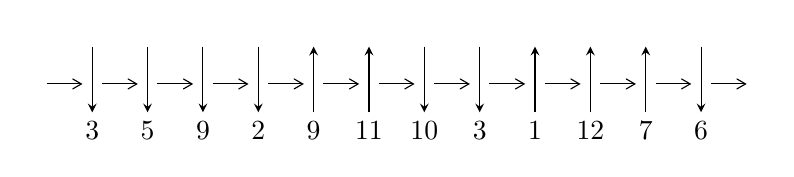
\begin{tikzpicture}[x=20pt, y=17pt]
	% nodes
	\node (C0) at (0, 0) {};
	\node (C1) at (1, 0) {};
	\node (C1U) at (1, +1) {};
	\node (C1D) at (1, -1) {3};

	\node (C2) at (2, 0) {};
	\node (C2U) at (2, +1) {};
	\node (C2D) at (2, -1) {5};

	\node (C3) at (3, 0) {};
	\node (C3U) at (3, +1) {};
	\node (C3D) at (3, -1) {9};

	\node (C4) at (4, 0) {};
	\node (C4U) at (4, +1) {};
	\node (C4D) at (4, -1) {2};

	\node (C5) at (5, 0) {};
	\node (C5U) at (5, +1) {};
	\node (C5D) at (5, -1) {9};

	\node (C6) at (6, 0) {};
	\node (C6U) at (6, +1) {};
	\node (C6D) at (6, -1) {11};

	\node (C7) at (7, 0) {};
	\node (C7U) at (7, +1) {};
	\node (C7D) at (7, -1) {10};

	\node (C8) at (8, 0) {};
	\node (C8U) at (8, +1) {};
	\node (C8D) at (8, -1) {3};

	\node (C9) at (9, 0) {};
	\node (C9U) at (9, +1) {};
	\node (C9D) at (9, -1) {1};

	\node (C10) at (10, 0) {};
	\node (C10U) at (10, +1) {};
	\node (C10D) at (10, -1) {12};

	\node (C11) at (11, 0) {};
	\node (C11U) at (11, +1) {};
	\node (C11D) at (11, -1) {7};

	\node (C12) at (12, 0) {};
	\node (C12U) at (12, +1) {};
	\node (C12D) at (12, -1) {6};
	\node (C13) at (13, 0) {};

	% arrows
	\draw[->,>={angle 60}]
	(C0) edge (C1) (C1) edge (C2) (C2) edge (C3) (C3) edge (C4) (C4) edge (C5) (C5) edge (C6) (C6) edge (C7) (C7) edge (C8) (C8) edge (C9) (C9) edge (C10) (C10) edge (C11) (C11) edge (C12) (C12) edge (C13) ;	\draw[->,>=stealth]
	(C1U) edge (C1D) (C2U) edge (C2D) (C3U) edge (C3D) (C4U) edge (C4D) (C5D) edge (C5U) (C6D) edge (C6U) (C7U) edge (C7D) (C8U) edge (C8D) (C9D) edge (C9U) (C10D) edge (C10U) (C11D) edge (C11U) (C12U) edge (C12D) ;
	\end{tikzpicture} \\
\hhline{~~} \\& 
\textbf{Solving Sequence} \\ \cline{2-2} 
 &
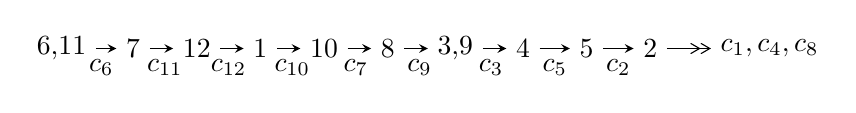
\begin{tikzpicture}[x=23pt, y=7pt]
	% node
	\node (A0) at (-1/8, 0) {6,11};
	\node (A1) at (1, 0) {7};
	\node (A2) at (2, 0) {12};
	\node (A3) at (3, 0) {1};
	\node (A4) at (4, 0) {10};
	\node (A5) at (5, 0) {8};
	\node (A6) at (97/16, 0) {3,9};
	\node (A7) at (57/8, 0) {4};
	\node (A8) at (65/8, 0) {5};
	\node (A9) at (73/8, 0) {2};
	\node (C1) at (1/2, -1) {$c_{6}$};
	\node (C2) at (3/2, -1) {$c_{11}$};
	\node (C3) at (5/2, -1) {$c_{12}$};
	\node (C4) at (7/2, -1) {$c_{10}$};
	\node (C5) at (9/2, -1) {$c_{7}$};
	\node (C6) at (11/2, -1) {$c_{9}$};
	\node (C7) at (53/8, -1) {$c_{3}$};
	\node (C8) at (61/8, -1) {$c_{5}$};
	\node (C9) at (69/8, -1) {$c_{2}$};
	\node (A10) at (11, 0) {$c_{1},c_{4},c_{8}$};

	% edge
	\draw[->,>=stealth]	
	(A0) edge (A1) (A1) edge (A2) (A2) edge (A3) (A3) edge (A4) (A4) edge (A5) (A5) edge (A6) (A6) edge (A7) (A7) edge (A8) (A8) edge (A9) ;
	\draw[->>,>={angle 60}]	
	(A9) edge (A10);
\end{tikzpicture} \\ 

\end{tabular} \\

\footnotetext{
The image of knot diagram is generated by the software ``\textbf{Draw programme}" developed by Andrew Bartholomew(\url{http://www.layer8.co.uk/maths/draw/index.htm\#Running-draw}), where we modified some parts for our purpose(\url{https://github.com/CATsTAILs/LinksPainter}).
}\phantom \\ \newline 
\centering \textbf{Ideals for irreducible components\footnotemark of $X_{\text{par}}$} 
 
\begin{align*}
I^u_{1}&=\langle 
- u^{50}- u^{49}+\cdots-4 u^2+b,\;-3 u^{50}-3 u^{49}+\cdots+a+4,\;u^{51}+2 u^{50}+\cdots+6 u^2-1\rangle \\
I^u_{2}&=\langle 
b+1,\;u^7-2 u^5+u^4+2 u^3- u^2+a+u,\;u^9- u^8-2 u^7+3 u^6+u^5-3 u^4+2 u^3- u+1\rangle \\
\\
\end{align*}
\raggedright * 2 irreducible components of $\dim_{\mathbb{C}}=0$, with total 60 representations.\\
\footnotetext{All coefficients of polynomials are rational numbers. But the coefficients are sometimes approximated in decimal forms when there is not enough margin.}
\newpage
\renewcommand{\arraystretch}{1}
\centering \section*{I. $I^u_{1}= \langle - u^{50}- u^{49}+\cdots-4 u^2+b,\;-3 u^{50}-3 u^{49}+\cdots+a+4,\;u^{51}+2 u^{50}+\cdots+6 u^2-1 \rangle$}
\flushleft \textbf{(i) Arc colorings}\\
\begin{tabular}{m{7pt} m{180pt} m{7pt} m{180pt} }
\flushright $a_{6}=$&$\begin{pmatrix}1\\0\end{pmatrix}$ \\
\flushright $a_{11}=$&$\begin{pmatrix}0\\u\end{pmatrix}$ \\
\flushright $a_{7}=$&$\begin{pmatrix}1\\- u^2\end{pmatrix}$ \\
\flushright $a_{12}=$&$\begin{pmatrix}u\\- u^3+u\end{pmatrix}$ \\
\flushright $a_{1}=$&$\begin{pmatrix}u^3\\- u^3+u\end{pmatrix}$ \\
\flushright $a_{10}=$&$\begin{pmatrix}- u^3\\u^5- u^3+u\end{pmatrix}$ \\
\flushright $a_{8}=$&$\begin{pmatrix}u^6- u^4+1\\- u^8+2 u^6-2 u^4\end{pmatrix}$ \\
\flushright $a_{3}=$&$\begin{pmatrix}3 u^{50}+3 u^{49}+\cdots+15 u^2-4\\u^{50}+u^{49}+\cdots+5 u^3+4 u^2\end{pmatrix}$ \\
\flushright $a_{9}=$&$\begin{pmatrix}- u^{11}+2 u^9-2 u^7- u^3\\u^{11}-3 u^9+4 u^7- u^5- u^3+u\end{pmatrix}$ \\
\flushright $a_{4}=$&$\begin{pmatrix}5 u^{50}+5 u^{49}+\cdots+22 u^2-5\\u^{50}+u^{49}+\cdots+5 u^2- u\end{pmatrix}$ \\
\flushright $a_{5}=$&$\begin{pmatrix}- u^{22}+5 u^{20}-12 u^{18}+15 u^{16}-10 u^{14}+2 u^{12}- u^8+u^6- u^4+1\\u^{22}-6 u^{20}+17 u^{18}-26 u^{16}+20 u^{14}-13 u^{10}+10 u^8- u^6-2 u^4+u^2\end{pmatrix}$ \\
\flushright $a_{2}=$&$\begin{pmatrix}2 u^{50}+2 u^{49}+\cdots+u-3\\u^{50}+u^{49}+\cdots+2 u^2+u\end{pmatrix}$\\&\end{tabular}
\flushleft \textbf{(ii) Obstruction class $= -1$}\\~\\
\flushleft \textbf{(iii) Cusp Shapes $= -10 u^{50}-13 u^{49}+\cdots-22 u+5$}\\~\\
\newpage\renewcommand{\arraystretch}{1}
\flushleft \textbf{(iv) u-Polynomials at the component}\newline \\
\begin{tabular}{m{50pt}|m{274pt}}
Crossings & \hspace{64pt}u-Polynomials at each crossing \\
\hline $$\begin{aligned}c_{1}\end{aligned}$$&$\begin{aligned}
&u^{51}+12 u^{50}+\cdots+8 u+1
\end{aligned}$\\
\hline $$\begin{aligned}c_{2},c_{4}\end{aligned}$$&$\begin{aligned}
&u^{51}-10 u^{50}+\cdots-8 u+1
\end{aligned}$\\
\hline $$\begin{aligned}c_{3},c_{8}\end{aligned}$$&$\begin{aligned}
&u^{51}+u^{50}+\cdots+512 u+512
\end{aligned}$\\
\hline $$\begin{aligned}c_{5}\end{aligned}$$&$\begin{aligned}
&u^{51}-2 u^{50}+\cdots+2 u+1
\end{aligned}$\\
\hline $$\begin{aligned}c_{6},c_{11}\end{aligned}$$&$\begin{aligned}
&u^{51}-2 u^{50}+\cdots-6 u^2+1
\end{aligned}$\\
\hline $$\begin{aligned}c_{7},c_{12}\end{aligned}$$&$\begin{aligned}
&u^{51}-6 u^{50}+\cdots-64 u+5
\end{aligned}$\\
\hline $$\begin{aligned}c_{9}\end{aligned}$$&$\begin{aligned}
&u^{51}+8 u^{50}+\cdots+20174 u-565
\end{aligned}$\\
\hline $$\begin{aligned}c_{10}\end{aligned}$$&$\begin{aligned}
&u^{51}-28 u^{50}+\cdots+12 u-1
\end{aligned}$\\
\hline
\end{tabular}\\~\\
\newpage\renewcommand{\arraystretch}{1}
\flushleft \textbf{(v) Riley Polynomials at the component}\newline \\
\begin{tabular}{m{50pt}|m{274pt}}
Crossings & \hspace{64pt}Riley Polynomials at each crossing \\
\hline $$\begin{aligned}c_{1}\end{aligned}$$&$\begin{aligned}
&y^{51}+64 y^{50}+\cdots+108 y-1
\end{aligned}$\\
\hline $$\begin{aligned}c_{2},c_{4}\end{aligned}$$&$\begin{aligned}
&y^{51}-12 y^{50}+\cdots+8 y-1
\end{aligned}$\\
\hline $$\begin{aligned}c_{3},c_{8}\end{aligned}$$&$\begin{aligned}
&y^{51}+57 y^{50}+\cdots-4194304 y-262144
\end{aligned}$\\
\hline $$\begin{aligned}c_{5}\end{aligned}$$&$\begin{aligned}
&y^{51}-60 y^{50}+\cdots+12 y-1
\end{aligned}$\\
\hline $$\begin{aligned}c_{6},c_{11}\end{aligned}$$&$\begin{aligned}
&y^{51}-28 y^{50}+\cdots+12 y-1
\end{aligned}$\\
\hline $$\begin{aligned}c_{7},c_{12}\end{aligned}$$&$\begin{aligned}
&y^{51}+44 y^{50}+\cdots+1176 y-25
\end{aligned}$\\
\hline $$\begin{aligned}c_{9}\end{aligned}$$&$\begin{aligned}
&y^{51}-24 y^{50}+\cdots+384067096 y-319225
\end{aligned}$\\
\hline $$\begin{aligned}c_{10}\end{aligned}$$&$\begin{aligned}
&y^{51}-8 y^{50}+\cdots+72 y-1
\end{aligned}$\\
\hline
\end{tabular}\\~\\
\newpage\flushleft \textbf{(vi) Complex Volumes and Cusp Shapes}
$$\begin{array}{c|c|c}  
\text{Solutions to }I^u_{1}& \I (\text{vol} + \sqrt{-1}CS) & \text{Cusp shape}\\
 \hline 
\begin{aligned}
u &= \phantom{-}0.870347 + 0.438821 I \\
a &= \phantom{-}0.015315 + 0.902084 I \\
b &= \phantom{-}0.136807 - 0.606788 I\end{aligned}
 & -0.59383 + 3.47183 I & -2.57465 - 7.94209 I \\ \hline\begin{aligned}
u &= \phantom{-}0.870347 - 0.438821 I \\
a &= \phantom{-}0.015315 - 0.902084 I \\
b &= \phantom{-}0.136807 + 0.606788 I\end{aligned}
 & -0.59383 - 3.47183 I & -2.57465 + 7.94209 I \\ \hline\begin{aligned}
u &= \phantom{-}0.769432 + 0.540134 I \\
a &= -0.334413 + 0.181071 I \\
b &= \phantom{-}0.262412 - 0.045879 I\end{aligned}
 & -2.41085 + 2.18056 I & -0.89273 - 4.14337 I \\ \hline\begin{aligned}
u &= \phantom{-}0.769432 - 0.540134 I \\
a &= -0.334413 - 0.181071 I \\
b &= \phantom{-}0.262412 + 0.045879 I\end{aligned}
 & -2.41085 - 2.18056 I & -0.89273 + 4.14337 I \\ \hline\begin{aligned}
u &= -0.918255 + 0.555689 I \\
a &= \phantom{-}2.35354 - 0.32507 I \\
b &= \phantom{-}0.33439 + 1.82533 I\end{aligned}
 & \phantom{-}4.75622 - 8.70313 I & -1.30654 + 7.99573 I \\ \hline\begin{aligned}
u &= -0.918255 - 0.555689 I \\
a &= \phantom{-}2.35354 + 0.32507 I \\
b &= \phantom{-}0.33439 - 1.82533 I\end{aligned}
 & \phantom{-}4.75622 + 8.70313 I & -1.30654 - 7.99573 I \\ \hline\begin{aligned}
u &= -0.961040 + 0.526565 I \\
a &= -2.26543 + 0.37900 I \\
b &= -0.19641 - 1.57019 I\end{aligned}
 & \phantom{-}5.41584 - 1.98677 I & \phantom{-0.000000 -}0. + 3.17688 I \\ \hline\begin{aligned}
u &= -0.961040 - 0.526565 I \\
a &= -2.26543 - 0.37900 I \\
b &= -0.19641 + 1.57019 I\end{aligned}
 & \phantom{-}5.41584 + 1.98677 I & \phantom{-0.000000 } 0. - 3.17688 I \\ \hline\begin{aligned}
u &= -0.892007 + 0.102900 I \\
a &= -0.782404 + 0.397432 I \\
b &= -0.1264520 - 0.0345198 I\end{aligned}
 & \phantom{-}1.50518 - 0.26567 I & \phantom{-}6.00026 + 0.27915 I \\ \hline\begin{aligned}
u &= -0.892007 - 0.102900 I \\
a &= -0.782404 - 0.397432 I \\
b &= -0.1264520 + 0.0345198 I\end{aligned}
 & \phantom{-}1.50518 + 0.26567 I & \phantom{-}6.00026 - 0.27915 I\\
 \hline 
 \end{array}$$\newpage$$\begin{array}{c|c|c}  
\text{Solutions to }I^u_{1}& \I (\text{vol} + \sqrt{-1}CS) & \text{Cusp shape}\\
 \hline 
\begin{aligned}
u &= \phantom{-}1.103930 + 0.029028 I \\
a &= \phantom{-}0.03014 + 2.74289 I \\
b &= \phantom{-}0.00205 - 1.91806 I\end{aligned}
 & \phantom{-}8.92371 + 3.58327 I & \phantom{-}4.99152 - 2.55707 I \\ \hline\begin{aligned}
u &= \phantom{-}1.103930 - 0.029028 I \\
a &= \phantom{-}0.03014 - 2.74289 I \\
b &= \phantom{-}0.00205 + 1.91806 I\end{aligned}
 & \phantom{-}8.92371 - 3.58327 I & \phantom{-}4.99152 + 2.55707 I \\ \hline\begin{aligned}
u &= -0.784529 + 0.412156 I \\
a &= \phantom{-}1.58952 - 1.83215 I \\
b &= \phantom{-}1.41941 + 0.12823 I\end{aligned}
 & -2.37641 - 1.79904 I & -1.57784 + 3.21479 I \\ \hline\begin{aligned}
u &= -0.784529 - 0.412156 I \\
a &= \phantom{-}1.58952 + 1.83215 I \\
b &= \phantom{-}1.41941 - 0.12823 I\end{aligned}
 & -2.37641 + 1.79904 I & -1.57784 - 3.21479 I \\ \hline\begin{aligned}
u &= -0.128537 + 0.840120 I \\
a &= \phantom{-}1.129030 + 0.709012 I \\
b &= \phantom{-}0.40430 - 2.07036 I\end{aligned}
 & \phantom{-}8.84070 + 9.07061 I & -0.40037 - 4.94351 I \\ \hline\begin{aligned}
u &= -0.128537 - 0.840120 I \\
a &= \phantom{-}1.129030 - 0.709012 I \\
b &= \phantom{-}0.40430 + 2.07036 I\end{aligned}
 & \phantom{-}8.84070 - 9.07061 I & -0.40037 + 4.94351 I \\ \hline\begin{aligned}
u &= -0.098639 + 0.843425 I \\
a &= -0.991418 - 0.802908 I \\
b &= -0.49696 + 1.82819 I\end{aligned}
 & \phantom{-}9.77996 + 1.74437 I & \phantom{-}0.869817 - 0.468289 I \\ \hline\begin{aligned}
u &= -0.098639 - 0.843425 I \\
a &= -0.991418 + 0.802908 I \\
b &= -0.49696 - 1.82819 I\end{aligned}
 & \phantom{-}9.77996 - 1.74437 I & \phantom{-}0.869817 + 0.468289 I \\ \hline\begin{aligned}
u &= -0.562511 + 0.604780 I \\
a &= -0.207632 - 1.106740 I \\
b &= \phantom{-}0.22739 - 1.74075 I\end{aligned}
 & \phantom{-}3.75359 + 4.13544 I & -3.29521 - 2.12817 I \\ \hline\begin{aligned}
u &= -0.562511 - 0.604780 I \\
a &= -0.207632 + 1.106740 I \\
b &= \phantom{-}0.22739 + 1.74075 I\end{aligned}
 & \phantom{-}3.75359 - 4.13544 I & -3.29521 + 2.12817 I\\
 \hline 
 \end{array}$$\newpage$$\begin{array}{c|c|c}  
\text{Solutions to }I^u_{1}& \I (\text{vol} + \sqrt{-1}CS) & \text{Cusp shape}\\
 \hline 
\begin{aligned}
u &= \phantom{-}0.071264 + 0.783310 I \\
a &= -0.318627 - 0.574074 I \\
b &= -0.332760 + 0.593277 I\end{aligned}
 & \phantom{-}2.40985 - 2.75947 I & \phantom{-}0.20281 + 3.78069 I \\ \hline\begin{aligned}
u &= \phantom{-}0.071264 - 0.783310 I \\
a &= -0.318627 + 0.574074 I \\
b &= -0.332760 - 0.593277 I\end{aligned}
 & \phantom{-}2.40985 + 2.75947 I & \phantom{-}0.20281 - 3.78069 I \\ \hline\begin{aligned}
u &= -1.159840 + 0.371143 I \\
a &= -0.819557 + 0.084078 I \\
b &= \phantom{-}0.146793 - 0.318351 I\end{aligned}
 & \phantom{-}3.81880 - 0.72340 I & \phantom{-0.000000 } 0 \\ \hline\begin{aligned}
u &= -1.159840 - 0.371143 I \\
a &= -0.819557 - 0.084078 I \\
b &= \phantom{-}0.146793 + 0.318351 I\end{aligned}
 & \phantom{-}3.81880 + 0.72340 I & \phantom{-0.000000 } 0 \\ \hline\begin{aligned}
u &= -0.481732 + 0.609553 I \\
a &= -0.101202 + 0.987549 I \\
b &= -0.01229 + 1.62632 I\end{aligned}
 & \phantom{-}4.06039 - 2.47774 I & -2.81595 + 2.59394 I \\ \hline\begin{aligned}
u &= -0.481732 - 0.609553 I \\
a &= -0.101202 - 0.987549 I \\
b &= -0.01229 - 1.62632 I\end{aligned}
 & \phantom{-}4.06039 + 2.47774 I & -2.81595 - 2.59394 I \\ \hline\begin{aligned}
u &= \phantom{-}0.173693 + 0.738661 I \\
a &= -0.367593 + 0.052677 I \\
b &= \phantom{-}0.234475 + 0.228624 I\end{aligned}
 & -0.01361 - 2.88077 I & \phantom{-}0.72874 + 4.09182 I \\ \hline\begin{aligned}
u &= \phantom{-}0.173693 - 0.738661 I \\
a &= -0.367593 - 0.052677 I \\
b &= \phantom{-}0.234475 - 0.228624 I\end{aligned}
 & -0.01361 + 2.88077 I & \phantom{-}0.72874 - 4.09182 I \\ \hline\begin{aligned}
u &= \phantom{-}1.182480 + 0.442140 I \\
a &= -1.75563 - 0.72377 I \\
b &= \phantom{-}1.24222 + 0.73561 I\end{aligned}
 & \phantom{-}3.09283 + 3.04460 I & \phantom{-0.000000 } 0 \\ \hline\begin{aligned}
u &= \phantom{-}1.182480 - 0.442140 I \\
a &= -1.75563 + 0.72377 I \\
b &= \phantom{-}1.24222 - 0.73561 I\end{aligned}
 & \phantom{-}3.09283 - 3.04460 I & \phantom{-0.000000 } 0\\
 \hline 
 \end{array}$$\newpage$$\begin{array}{c|c|c}  
\text{Solutions to }I^u_{1}& \I (\text{vol} + \sqrt{-1}CS) & \text{Cusp shape}\\
 \hline 
\begin{aligned}
u &= \phantom{-}0.654402 + 0.333690 I \\
a &= -1.061450 - 0.491092 I \\
b &= \phantom{-}0.509880 + 0.457534 I\end{aligned}
 & -1.277320 + 0.104972 I & -6.49712 - 0.81478 I \\ \hline\begin{aligned}
u &= \phantom{-}0.654402 - 0.333690 I \\
a &= -1.061450 + 0.491092 I \\
b &= \phantom{-}0.509880 - 0.457534 I\end{aligned}
 & -1.277320 - 0.104972 I & -6.49712 + 0.81478 I \\ \hline\begin{aligned}
u &= \phantom{-}1.164800 + 0.508279 I \\
a &= -0.311275 + 0.409745 I \\
b &= \phantom{-}0.287422 - 0.271809 I\end{aligned}
 & \phantom{-}2.86161 + 7.55446 I & \phantom{-0.000000 } 0 \\ \hline\begin{aligned}
u &= \phantom{-}1.164800 - 0.508279 I \\
a &= -0.311275 - 0.409745 I \\
b &= \phantom{-}0.287422 + 0.271809 I\end{aligned}
 & \phantom{-}2.86161 - 7.55446 I & \phantom{-0.000000 } 0 \\ \hline\begin{aligned}
u &= -1.183710 + 0.466863 I \\
a &= -0.43063 - 2.86734 I \\
b &= \phantom{-}1.42604 + 0.63435 I\end{aligned}
 & \phantom{-}2.91319 - 5.51229 I & \phantom{-0.000000 } 0 \\ \hline\begin{aligned}
u &= -1.183710 - 0.466863 I \\
a &= -0.43063 + 2.86734 I \\
b &= \phantom{-}1.42604 - 0.63435 I\end{aligned}
 & \phantom{-}2.91319 + 5.51229 I & \phantom{-0.000000 } 0 \\ \hline\begin{aligned}
u &= -0.040008 + 0.724234 I \\
a &= \phantom{-}0.167745 + 1.283370 I \\
b &= \phantom{-}1.29438 - 0.57599 I\end{aligned}
 & -0.344586 + 1.125350 I & -2.18776 + 0.36560 I \\ \hline\begin{aligned}
u &= -0.040008 - 0.724234 I \\
a &= \phantom{-}0.167745 - 1.283370 I \\
b &= \phantom{-}1.29438 + 0.57599 I\end{aligned}
 & -0.344586 - 1.125350 I & -2.18776 - 0.36560 I \\ \hline\begin{aligned}
u &= -1.205000 + 0.421939 I \\
a &= -0.336159 + 1.363990 I \\
b &= -0.446127 - 0.523396 I\end{aligned}
 & \phantom{-}6.14415 - 1.44415 I & \phantom{-0.000000 } 0 \\ \hline\begin{aligned}
u &= -1.205000 - 0.421939 I \\
a &= -0.336159 - 1.363990 I \\
b &= -0.446127 + 0.523396 I\end{aligned}
 & \phantom{-}6.14415 + 1.44415 I & \phantom{-0.000000 } 0\\
 \hline 
 \end{array}$$\newpage$$\begin{array}{c|c|c}  
\text{Solutions to }I^u_{1}& \I (\text{vol} + \sqrt{-1}CS) & \text{Cusp shape}\\
 \hline 
\begin{aligned}
u &= \phantom{-}1.199230 + 0.483275 I \\
a &= \phantom{-}0.623123 + 0.813683 I \\
b &= -0.381068 - 0.691428 I\end{aligned}
 & \phantom{-}5.70689 + 7.38464 I & \phantom{-0.000000 } 0 \\ \hline\begin{aligned}
u &= \phantom{-}1.199230 - 0.483275 I \\
a &= \phantom{-}0.623123 - 0.813683 I \\
b &= -0.381068 + 0.691428 I\end{aligned}
 & \phantom{-}5.70689 - 7.38464 I & \phantom{-0.000000 } 0 \\ \hline\begin{aligned}
u &= \phantom{-}1.236290 + 0.382809 I \\
a &= -0.78559 - 2.71496 I \\
b &= \phantom{-}0.35139 + 2.12412 I\end{aligned}
 & \phantom{-}13.00930 - 4.90240 I & \phantom{-0.000000 } 0 \\ \hline\begin{aligned}
u &= \phantom{-}1.236290 - 0.382809 I \\
a &= -0.78559 + 2.71496 I \\
b &= \phantom{-}0.35139 - 2.12412 I\end{aligned}
 & \phantom{-}13.00930 + 4.90240 I & \phantom{-0.000000 } 0 \\ \hline\begin{aligned}
u &= \phantom{-}1.238740 + 0.402230 I \\
a &= \phantom{-}0.91998 + 2.41477 I \\
b &= -0.47327 - 1.91914 I\end{aligned}
 & \phantom{-}13.84570 + 2.55616 I & \phantom{-0.000000 } 0 \\ \hline\begin{aligned}
u &= \phantom{-}1.238740 - 0.402230 I \\
a &= \phantom{-}0.91998 - 2.41477 I \\
b &= -0.47327 + 1.91914 I\end{aligned}
 & \phantom{-}13.84570 - 2.55616 I & \phantom{-0.000000 } 0 \\ \hline\begin{aligned}
u &= -1.209920 + 0.515926 I \\
a &= \phantom{-}2.42150 - 2.66691 I \\
b &= \phantom{-}0.45186 + 2.09789 I\end{aligned}
 & \phantom{-}12.0604 - 14.0151 I & \phantom{-0.000000 } 0 \\ \hline\begin{aligned}
u &= -1.209920 - 0.515926 I \\
a &= \phantom{-}2.42150 + 2.66691 I \\
b &= \phantom{-}0.45186 - 2.09789 I\end{aligned}
 & \phantom{-}12.0604 + 14.0151 I & \phantom{-0.000000 } 0 \\ \hline\begin{aligned}
u &= -1.217650 + 0.504060 I \\
a &= -1.94270 + 2.65801 I \\
b &= -0.57244 - 1.82873 I\end{aligned}
 & \phantom{-}13.1170 - 6.6351 I & \phantom{-0.000000 } 0 \\ \hline\begin{aligned}
u &= -1.217650 - 0.504060 I \\
a &= -1.94270 - 2.65801 I \\
b &= -0.57244 + 1.82873 I\end{aligned}
 & \phantom{-}13.1170 + 6.6351 I & \phantom{-0.000000 } 0\\
 \hline 
 \end{array}$$\newpage$$\begin{array}{c|c|c}  
\text{Solutions to }I^u_{1}& \I (\text{vol} + \sqrt{-1}CS) & \text{Cusp shape}\\
 \hline 
\begin{aligned}
u &= \phantom{-}0.357516\phantom{ +0.000000I} \\
a &= -1.87639\phantom{ +0.000000I} \\
b &= \phantom{-}0.613111\phantom{ +0.000000I}\end{aligned}
 & -1.12692\phantom{ +0.000000I} & -9.48630\phantom{ +0.000000I}\\
 \hline 
 \end{array}$$\newpage\newpage\renewcommand{\arraystretch}{1}
\centering \section*{II. $I^u_{2}= \langle b+1,\;u^7-2 u^5+u^4+2 u^3- u^2+a+u,\;u^9- u^8-2 u^7+3 u^6+u^5-3 u^4+2 u^3- u+1 \rangle$}
\flushleft \textbf{(i) Arc colorings}\\
\begin{tabular}{m{7pt} m{180pt} m{7pt} m{180pt} }
\flushright $a_{6}=$&$\begin{pmatrix}1\\0\end{pmatrix}$ \\
\flushright $a_{11}=$&$\begin{pmatrix}0\\u\end{pmatrix}$ \\
\flushright $a_{7}=$&$\begin{pmatrix}1\\- u^2\end{pmatrix}$ \\
\flushright $a_{12}=$&$\begin{pmatrix}u\\- u^3+u\end{pmatrix}$ \\
\flushright $a_{1}=$&$\begin{pmatrix}u^3\\- u^3+u\end{pmatrix}$ \\
\flushright $a_{10}=$&$\begin{pmatrix}- u^3\\u^5- u^3+u\end{pmatrix}$ \\
\flushright $a_{8}=$&$\begin{pmatrix}u^6- u^4+1\\- u^8+2 u^6-2 u^4\end{pmatrix}$ \\
\flushright $a_{3}=$&$\begin{pmatrix}- u^7+2 u^5- u^4-2 u^3+u^2- u\\-1\end{pmatrix}$ \\
\flushright $a_{9}=$&$\begin{pmatrix}u^6- u^4+1\\- u^8+2 u^6-2 u^4\end{pmatrix}$ \\
\flushright $a_{4}=$&$\begin{pmatrix}- u^7+2 u^5- u^4-2 u^3+u^2- u\\-1\end{pmatrix}$ \\
\flushright $a_{5}=$&$\begin{pmatrix}- u^3\\u^3- u\end{pmatrix}$ \\
\flushright $a_{2}=$&$\begin{pmatrix}- u^7+2 u^5- u^4- u^3+u^2- u\\- u^3+u-1\end{pmatrix}$\\&\end{tabular}
\flushleft \textbf{(ii) Obstruction class $= 1$}\\~\\
\flushleft \textbf{(iii) Cusp Shapes $= u^8-6 u^7- u^6+12 u^5-5 u^4-10 u^3+7 u^2-7 u-6$}\\~\\
\newpage\renewcommand{\arraystretch}{1}
\flushleft \textbf{(iv) u-Polynomials at the component}\newline \\
\begin{tabular}{m{50pt}|m{274pt}}
Crossings & \hspace{64pt}u-Polynomials at each crossing \\
\hline $$\begin{aligned}c_{1},c_{2}\end{aligned}$$&$\begin{aligned}
&(u-1)^9
\end{aligned}$\\
\hline $$\begin{aligned}c_{3},c_{8}\end{aligned}$$&$\begin{aligned}
&u^9
\end{aligned}$\\
\hline $$\begin{aligned}c_{4}\end{aligned}$$&$\begin{aligned}
&(u+1)^9
\end{aligned}$\\
\hline $$\begin{aligned}c_{5},c_{9}\end{aligned}$$&$\begin{aligned}
&u^9- u^8+2 u^7- u^6+3 u^5- u^4+2 u^3+u+1
\end{aligned}$\\
\hline $$\begin{aligned}c_{6}\end{aligned}$$&$\begin{aligned}
&u^9- u^8-2 u^7+3 u^6+u^5-3 u^4+2 u^3- u+1
\end{aligned}$\\
\hline $$\begin{aligned}c_{7}\end{aligned}$$&$\begin{aligned}
&u^9-3 u^8+8 u^7-13 u^6+17 u^5-17 u^4+12 u^3-6 u^2+u+1
\end{aligned}$\\
\hline $$\begin{aligned}c_{10}\end{aligned}$$&$\begin{aligned}
&u^9+5 u^8+12 u^7+15 u^6+9 u^5- u^4-4 u^3-2 u^2+u+1
\end{aligned}$\\
\hline $$\begin{aligned}c_{11}\end{aligned}$$&$\begin{aligned}
&u^9+u^8-2 u^7-3 u^6+u^5+3 u^4+2 u^3- u-1
\end{aligned}$\\
\hline $$\begin{aligned}c_{12}\end{aligned}$$&$\begin{aligned}
&u^9+3 u^8+8 u^7+13 u^6+17 u^5+17 u^4+12 u^3+6 u^2+u-1
\end{aligned}$\\
\hline
\end{tabular}\\~\\
\newpage\renewcommand{\arraystretch}{1}
\flushleft \textbf{(v) Riley Polynomials at the component}\newline \\
\begin{tabular}{m{50pt}|m{274pt}}
Crossings & \hspace{64pt}Riley Polynomials at each crossing \\
\hline $$\begin{aligned}c_{1},c_{2},c_{4}\end{aligned}$$&$\begin{aligned}
&(y-1)^9
\end{aligned}$\\
\hline $$\begin{aligned}c_{3},c_{8}\end{aligned}$$&$\begin{aligned}
&y^9
\end{aligned}$\\
\hline $$\begin{aligned}c_{5},c_{9}\end{aligned}$$&$\begin{aligned}
&y^9+3 y^8+8 y^7+13 y^6+17 y^5+17 y^4+12 y^3+6 y^2+y-1
\end{aligned}$\\
\hline $$\begin{aligned}c_{6},c_{11}\end{aligned}$$&$\begin{aligned}
&y^9-5 y^8+12 y^7-15 y^6+9 y^5+y^4-4 y^3+2 y^2+y-1
\end{aligned}$\\
\hline $$\begin{aligned}c_{7},c_{12}\end{aligned}$$&$\begin{aligned}
&y^9+7 y^8+20 y^7+25 y^6+5 y^5-15 y^4+22 y^2+13 y-1
\end{aligned}$\\
\hline $$\begin{aligned}c_{10}\end{aligned}$$&$\begin{aligned}
&y^9- y^8+12 y^7-7 y^6+37 y^5+y^4-10 y^2+5 y-1
\end{aligned}$\\
\hline
\end{tabular}\\~\\
\newpage\flushleft \textbf{(vi) Complex Volumes and Cusp Shapes}
$$\begin{array}{c|c|c}  
\text{Solutions to }I^u_{2}& \I (\text{vol} + \sqrt{-1}CS) & \text{Cusp shape}\\
 \hline 
\begin{aligned}
u &= \phantom{-}0.772920 + 0.510351 I \\
a &= -0.628748 - 1.040710 I \\
b &= -1.00000\phantom{ +0.000000I}\end{aligned}
 & -3.42837 + 2.09337 I & -10.43453 - 4.18932 I \\ \hline\begin{aligned}
u &= \phantom{-}0.772920 - 0.510351 I \\
a &= -0.628748 + 1.040710 I \\
b &= -1.00000\phantom{ +0.000000I}\end{aligned}
 & -3.42837 - 2.09337 I & -10.43453 + 4.18932 I \\ \hline\begin{aligned}
u &= -0.825933\phantom{ +0.000000I} \\
a &= \phantom{-}1.66309\phantom{ +0.000000I} \\
b &= -1.00000\phantom{ +0.000000I}\end{aligned}
 & -0.446489\phantom{ +0.000000I} & \phantom{-}4.72420\phantom{ +0.000000I} \\ \hline\begin{aligned}
u &= -1.173910 + 0.391555 I \\
a &= \phantom{-}1.321020 + 0.175437 I \\
b &= -1.00000\phantom{ +0.000000I}\end{aligned}
 & \phantom{-}2.72642 - 1.33617 I & -0.549708 + 1.017936 I \\ \hline\begin{aligned}
u &= -1.173910 - 0.391555 I \\
a &= \phantom{-}1.321020 - 0.175437 I \\
b &= -1.00000\phantom{ +0.000000I}\end{aligned}
 & \phantom{-}2.72642 + 1.33617 I & -0.549708 - 1.017936 I \\ \hline\begin{aligned}
u &= \phantom{-}0.141484 + 0.739668 I \\
a &= \phantom{-}0.081981 + 0.728244 I \\
b &= -1.00000\phantom{ +0.000000I}\end{aligned}
 & -1.02799 - 2.45442 I & -6.31821 + 2.62939 I \\ \hline\begin{aligned}
u &= \phantom{-}0.141484 - 0.739668 I \\
a &= \phantom{-}0.081981 - 0.728244 I \\
b &= -1.00000\phantom{ +0.000000I}\end{aligned}
 & -1.02799 + 2.45442 I & -6.31821 - 2.62939 I \\ \hline\begin{aligned}
u &= \phantom{-}1.172470 + 0.500383 I \\
a &= \phantom{-}0.89420 - 1.47834 I \\
b &= -1.00000\phantom{ +0.000000I}\end{aligned}
 & \phantom{-}1.95319 + 7.08493 I & -3.05967 - 5.11095 I \\ \hline\begin{aligned}
u &= \phantom{-}1.172470 - 0.500383 I \\
a &= \phantom{-}0.89420 + 1.47834 I \\
b &= -1.00000\phantom{ +0.000000I}\end{aligned}
 & \phantom{-}1.95319 - 7.08493 I & -3.05967 + 5.11095 I\\
 \hline 
 \end{array}$$\newpage
\newpage\renewcommand{\arraystretch}{1}
\centering \section*{ III. u-Polynomials}
\begin{tabular}{m{50pt}|m{274pt}}
Crossings & \hspace{64pt}u-Polynomials at each crossing \\
\hline $$\begin{aligned}c_{1}\end{aligned}$$&$\begin{aligned}
&((u-1)^9)(u^{51}+12 u^{50}+\cdots+8 u+1)
\end{aligned}$\\
\hline $$\begin{aligned}c_{2}\end{aligned}$$&$\begin{aligned}
&((u-1)^9)(u^{51}-10 u^{50}+\cdots-8 u+1)
\end{aligned}$\\
\hline $$\begin{aligned}c_{3},c_{8}\end{aligned}$$&$\begin{aligned}
&u^9(u^{51}+u^{50}+\cdots+512 u+512)
\end{aligned}$\\
\hline $$\begin{aligned}c_{4}\end{aligned}$$&$\begin{aligned}
&((u+1)^9)(u^{51}-10 u^{50}+\cdots-8 u+1)
\end{aligned}$\\
\hline $$\begin{aligned}c_{5}\end{aligned}$$&$\begin{aligned}
&(u^9- u^8+\cdots+u+1)(u^{51}-2 u^{50}+\cdots+2 u+1)
\end{aligned}$\\
\hline $$\begin{aligned}c_{6}\end{aligned}$$&$\begin{aligned}
&(u^9- u^8+\cdots- u+1)(u^{51}-2 u^{50}+\cdots-6 u^2+1)
\end{aligned}$\\
\hline $$\begin{aligned}c_{7}\end{aligned}$$&$\begin{aligned}
&(u^9-3 u^8+8 u^7-13 u^6+17 u^5-17 u^4+12 u^3-6 u^2+u+1)\\
&\cdot(u^{51}-6 u^{50}+\cdots-64 u+5)
\end{aligned}$\\
\hline $$\begin{aligned}c_{9}\end{aligned}$$&$\begin{aligned}
&(u^9- u^8+2 u^7- u^6+3 u^5- u^4+2 u^3+u+1)\\
&\cdot(u^{51}+8 u^{50}+\cdots+20174 u-565)
\end{aligned}$\\
\hline $$\begin{aligned}c_{10}\end{aligned}$$&$\begin{aligned}
&(u^9+5 u^8+12 u^7+15 u^6+9 u^5- u^4-4 u^3-2 u^2+u+1)\\
&\cdot(u^{51}-28 u^{50}+\cdots+12 u-1)
\end{aligned}$\\
\hline $$\begin{aligned}c_{11}\end{aligned}$$&$\begin{aligned}
&(u^9+u^8+\cdots- u-1)(u^{51}-2 u^{50}+\cdots-6 u^2+1)
\end{aligned}$\\
\hline $$\begin{aligned}c_{12}\end{aligned}$$&$\begin{aligned}
&(u^9+3 u^8+8 u^7+13 u^6+17 u^5+17 u^4+12 u^3+6 u^2+u-1)\\
&\cdot(u^{51}-6 u^{50}+\cdots-64 u+5)
\end{aligned}$\\
\hline
\end{tabular}\newpage\renewcommand{\arraystretch}{1}
\centering \section*{ IV. Riley Polynomials}
\begin{tabular}{m{50pt}|m{274pt}}
Crossings & \hspace{64pt}Riley Polynomials at each crossing \\
\hline $$\begin{aligned}c_{1}\end{aligned}$$&$\begin{aligned}
&((y-1)^9)(y^{51}+64 y^{50}+\cdots+108 y-1)
\end{aligned}$\\
\hline $$\begin{aligned}c_{2},c_{4}\end{aligned}$$&$\begin{aligned}
&((y-1)^9)(y^{51}-12 y^{50}+\cdots+8 y-1)
\end{aligned}$\\
\hline $$\begin{aligned}c_{3},c_{8}\end{aligned}$$&$\begin{aligned}
&y^9(y^{51}+57 y^{50}+\cdots-4194304 y-262144)
\end{aligned}$\\
\hline $$\begin{aligned}c_{5}\end{aligned}$$&$\begin{aligned}
&(y^9+3 y^8+8 y^7+13 y^6+17 y^5+17 y^4+12 y^3+6 y^2+y-1)\\
&\cdot(y^{51}-60 y^{50}+\cdots+12 y-1)
\end{aligned}$\\
\hline $$\begin{aligned}c_{6},c_{11}\end{aligned}$$&$\begin{aligned}
&(y^9-5 y^8+12 y^7-15 y^6+9 y^5+y^4-4 y^3+2 y^2+y-1)\\
&\cdot(y^{51}-28 y^{50}+\cdots+12 y-1)
\end{aligned}$\\
\hline $$\begin{aligned}c_{7},c_{12}\end{aligned}$$&$\begin{aligned}
&(y^9+7 y^8+20 y^7+25 y^6+5 y^5-15 y^4+22 y^2+13 y-1)\\
&\cdot(y^{51}+44 y^{50}+\cdots+1176 y-25)
\end{aligned}$\\
\hline $$\begin{aligned}c_{9}\end{aligned}$$&$\begin{aligned}
&(y^9+3 y^8+8 y^7+13 y^6+17 y^5+17 y^4+12 y^3+6 y^2+y-1)\\
&\cdot(y^{51}-24 y^{50}+\cdots+384067096 y-319225)
\end{aligned}$\\
\hline $$\begin{aligned}c_{10}\end{aligned}$$&$\begin{aligned}
&(y^9- y^8+12 y^7-7 y^6+37 y^5+y^4-10 y^2+5 y-1)\\
&\cdot(y^{51}-8 y^{50}+\cdots+72 y-1)
\end{aligned}$\\
\hline
\end{tabular}
\vskip 2pc
\end{document}